\documentclass{report}
\usepackage[utf8]{inputenc}
\usepackage{graphics}
\graphicspath{ {./images/} }
\usepackage{multicol}
\usepackage{array}

% width,height
\usepackage[a4paper, total={7in, 10in}]{geometry}

\title{OE - Assignment}
\author{ABARAJITH S}
\date{\today}

\begin{document}

    \begin{titlepage}
    \centering
        \vspace*{2cm}
        \Huge
        \textbf{IOT BASED SMART FOOD MONITORING SYSTEM}
        
        \vspace*{0.6cm}
        \Large
        \textit{}
        
        \normalsize
        \vspace*{1.5cm}
        ABARAJITH S\\
        \vspace{0.2cm}
        21011101004\\
        \vspace{0.2cm}
        AI-DS A\\
        
        \vfill     
        
        
\includegraphics{images/titleimg.jpeg}\\
        
        \vfill
        
        
\includegraphics{images/logo.jpg}\\
        Computer Science and Engineering\\
        Shiv Nadar University, Chennai\\
        20 January 2023
        \vspace*{1cm}
    
\end{titlepage}

    
    \begin{center}
        \section*{IOT BASED SMART FOOD MONITORING SYSTEM}
    \end{center}
\setlength{\columnsep}{1.0cm}
    \large
    \section*{Summary}
    Food safety and hygiene are among the key concerns in order to prevent the wastage of food. However, for lack of technology and ignorance about the effects of humidity, temperature, exposure to light and alcohol content on foods, food safety is not maintained well enough in Kenya. This has led to massive losses in many food stores resulting from food decay.
    Currently, majority of food stores and warehouses still rely on manual monitoring of the atmospheric factors related to food quality. These conventional food inspection technologies are limited to weight, volume, color and aspect inspection and as a result do not provide a lot of information needed on quality of food. The quality of the food needs to be monitored and it must be prevented from rotting and decaying by the atmospheric factors like temperature, humidity and dark.
    This project is focused on such a food monitoring system which suggests systematic use of various sensors to perform quality monitoring and control of food materials. More precisely, this system consists of gas, temperature, light and humidity sensors, which provide the essential information needed for evaluating the quality of the packed or stored product. This information is transmitted wirelessly to a computer system providing an interface where the user can observe the evolution of the product quality over time using the Internet of Things technology. Later, the environmental factors can be controlled like by refrigeration, vacuum storage and other appropriate control measures.
    
\begin{multicols}{1}    
    \section*{Introduction}
    The food we consume can affect in any form of contamination that may occur due to storage or chemical changes within the food. There are several viruses and bacteria that causes food contamination and leads to numerous food borne diseases, for example Norovirus a very contagious virus caused by contaminated food or water. About 351,000 people die of food poisoning globally every year. 
    In some countries, majority of people struggles on daily basis for food, due to preservation of foods and use of chemicals to artificially increase the time span of food causes people illness. It is necessary to develop a system that can help people to identify the freshness of food or quality of food items. Our proposed system may give the good quality (freshness) management in food. It is based on electrical, and biosensors. Biosensors play a vital role to detect the bacterial contamination in food sample. Based on the combination of the sensor outputs quality of the food should be detected.
    The existing system just does the work of monitoring the food through the temperature, humidity and light sensors. The increase in temperature suddenly may increase the risk of spoiling of the food. The increase in humidity may cause the damage of some type of the foods. Hence threshold values of the foods are set within which the food remains unspoilt. Other than temperature and humidity, the light also plays an important role. Lack of sufficient light to the food may cause it to spoil. Hence,artificial lights are made on, whenever the light is found insufficient through the sensor inputs turned into the analog values.
    The amount of the gas level released from the food is monitored through the gas sensors and converted into analog values to be displayed on the IoT platform to be monitored wherever required.However, different types of foods emit different types of gases when at the merge of getting spoilt. Further research is needed to be done in this context and the sensors are needed to be used accordingly.
   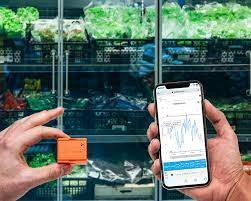
\includegraphics{images/monitor.jpeg}
    

    \section*{Block Diagram}
    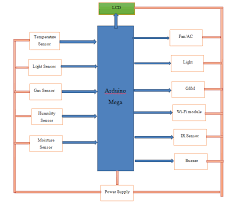
\includegraphics{images/blockdig.png}\\
    \section*{Working}
    We have wireless sensor unit to monitor the critical environmental parameters like temperature, humidity, light, moisture etc. we have DHT-11 sensor which will senses the humidity and temperature at shopping mall and give it to the Arduino. Arduino will convert this analog vale into digital value compared threshold value. If the parameter above or below the threshold value then actuators will turn on and control the temperature. Alarm will be on to turn on. We have gas sensor which will send message to owner. We have IR sensorunit, which is used to monitor the stock. If the stock is less it will sense and send information to the vendor.(Automatic ordering system). We have GSM to communicate with vendor and owner. We have EPS-8266(wi-fi)module which is used to upload all measured data into the cloud. We use Thing speak cloud, which is freely available for students. Which will collect the sent data and plot the graph. We can take daily /weekly/monthly report for data analysis. We have LCD display, which displays the status of each sensor.
    \scalebox{0.3}{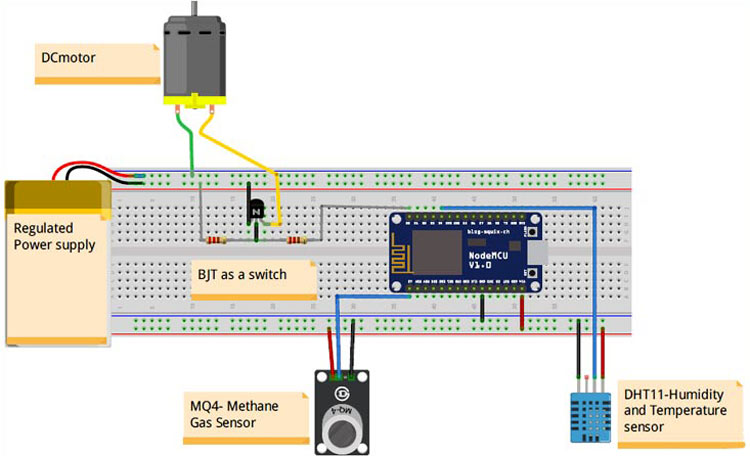
\includegraphics{images/CircuitDig.jpeg}}
    \section*{Hardware Requirment:}
    \begin{enumerate}
    \item Arduino mega
    \item ESP-8266 wi-fi module
    \item GSM800
    \item 16*2 LCD
    \item DHT-11 Sensor
    \item Ch4 Sensor
    \item Light Sensor
    \item Light 
    \item Fan
    \item Buzzer
    \item Humidity sensor
        
    \end{enumerate}
 
    \section*{Software Requirments}
    \begin{enumerate}
        \item Embedded C
        \item Arduino Sketch
        \item Thingspeak 
    \end{enumerate}

    \section*{Implementation}
    IoT device should be installed in a food store. Once it is properly installed and powered on, it connects with the internet via Wi-Fi modem and start reading data from the interfaced sensors- DHT-11 temperature and humidity sensor and LDR sensor. DHT11 temperature and humidity sensor is a digital sensor with inbuilt capactive humidity sensor and thermistor it realys a real- time temperature and humidity reading every 2 seconds. The sensors operators on 3.5 to 5.5 V supply and can read temperature between 0 degree C and 50 degree C and relative humidity between 20\% and 95\%.
    
    Sensor cannot be directly interfaced to a digital pin of the board as it operates on 1-wire protocol which must be implemented only on the firmware. The first data pin is configured to input and a start signal is sent to it. The start signal comprises of a LOW for 18 milliseconds followed by a HIGH for 20 to 40 microseconds followed by a LOW again for 80 microseconds and a HIGH for 80 microseconds. After sending the start signal, the pin is configured to digital output and 40-bit data comprising of the temperature and humidity reading is latched out. Of the 5-byte data, the first two bytes are integer and decimal part of reading for relative humidity respectively, third and fourth bytes are integer and decimal part of reading for temperature and last one is checksum byte.
    
    The LDR sensor is connected in a potential divider circuit and inputs a voltage at the analog input pin of the controller. The voltage is read and digitized using in-built ADC channel. The Arduino collects data from all the sensors and convert the values to the strings. The sensor data wrapped as proper strings are passed to the character LCD for display. The ESP8266 Wi-Fi module connected to the Arduino uploads the data to Cloud Server. For displaying and monitoring data uploaded to the Colud server, The analog output is passed to the analog pin of the Arduino which has inbuilt ADC that coverts the analog to digital value. 
    
    Today’s smart devices peripherals are becoming more integrated and play an important part of our computing experience and also offers the convenience of wireless connectivity, selection the sensor typically depends on blancing high performance against design complexity and board space, blancing ease of use against design complexity and cost, blancing high functionality against low-power consumption, cost savings and low space requirements.
    
    We have wireless sensor unit to monitor the critical environmental parameters like temperature, humidity, light, moisture etc. we have DHT-11 sensor which will senses the humidity and temperature at shopping mall and give it to the Arduino. Arduino will convert this analog vale into digital value compared threshold value. If the parameter above or below the threshold value then actuators will turn on and control the temperature. Alarm will be on to turn on. We have gas sensor which will send message to owner. We have IR sensor unit, which is used to monitor the stock. If the stock is less it will sense and send information to the vendor.

    We have GSM to communicate with vendor and owner. We have EPS-8266(wi-fi)module which is used to upload all measured data into the cloud. We use Thing speak cloud, which is freely available for students. Which will collect the sent data and plot the graph. We can take daily /weekly/monthly report for data analysis. We have LCD display, which displays the status of each sensor LDR Sensor - The LDR is used to sense the intensity of light. The sensor is connected to the A1 pin of the Arduino board. The sensor is connected in a potential divider circuit.
    
    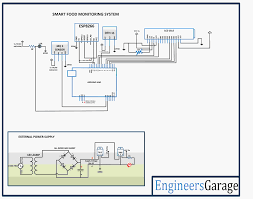
\includegraphics{images/Arduino.png }
 \section*{System Protocols :} 
    \scalebox{0.25}{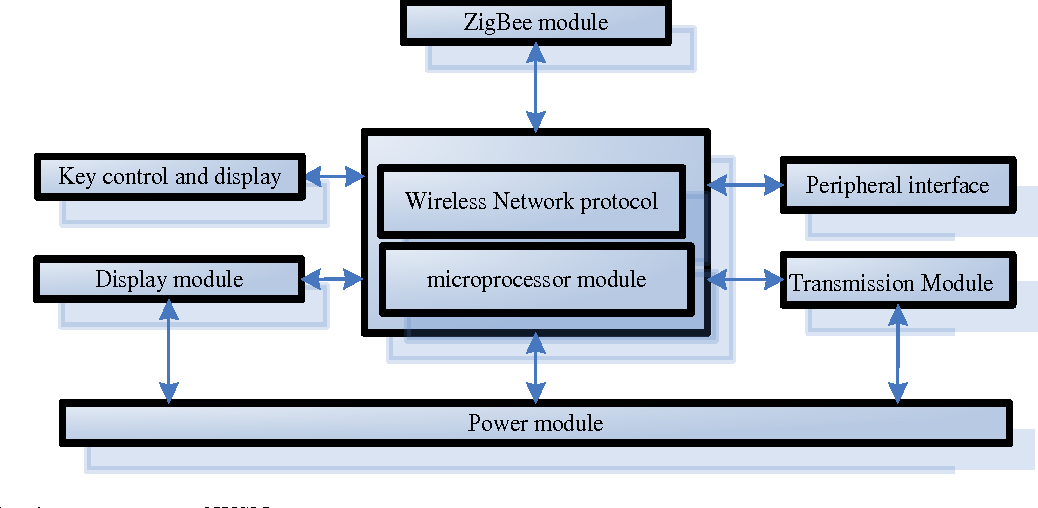
\includegraphics{images/protocal.png}}

    \section*{The ESP-01 model has the following pin configuration:} 
    \begin{center}
    \begin{tabular}{ | m{1em} | m{4em} | m{5cm} |}
    \hline
    \textbf 1 & Ground & Ground \\ 
    \hline
     2 & GPIO1 & General purpose IO,Serial Tx1\\ 
    \hline
     3 & GPIO2 & General purpose IO\\ 
    \hline
     4 & CHPD & Active High chip enable\\
    \hline
     5 & GPIO0 & General purpose IO,launch serial programming mode if low while reset or power ON\\
    \hline
     6 & RESET & Active Low External Reset Signal\\
    \hline
     7 & GPIO3 & General purpose IO,Serial Rx\\
    \hline
     8 & VCC & Power Supply\\
    \hline

    \end{tabular}
    \end{center}

    

        \section*{Advantages}
    \begin{itemize}
        \item Save fruits and vegetables for longer time.
        \item Maintain hygiene and clean environment.
        \item Save data into cloud for future analysis.
        \item Reduce the commercial loss.
        \item Increase commercial profit.
    \end{itemize}
    \section*{Applications}
    \begin{itemize}
        \item Can use this system in fruits and vegetable shops.
        \item Can use this system in agriculture farm.
        \item Can use this system in flower shops.
    \end{itemize}
     
    \section*{Conclusion}
   An IoT-based food monitoring system is a system that uses internet-connected devices to monitor and track food storage and consumption. This can include sensors placed in refrigerators and pantries to track the temperature and humidity of stored food, as well as cameras and other devices to track the movement and consumption of food. The data collected by these devices can then be analyzed and used to optimize food storage and consumption, reduce waste, and improve overall food safety. Additionally, it could be connected to a smart phone application to monitor and track the food consumption and provide recommendations.

  
    
\end{multicols}
\end{document}

